\documentclass[11pt]{beamer}
\usetheme{Warsaw}
\usepackage[utf8]{inputenc}
\usepackage{amsmath}
\usepackage{amsfonts}
\usepackage{amssymb}
\usepackage{multicol}

\author{Theofilos Papapanagiotou, Hung Nguyen}
\title{Sudoku SAT solver}
%\setbeamercovered{transparent}
%\setbeamertemplate{navigation symbols}{}
%\logo{}
\institute{UvA/VU}
%\date{}
%\subject{}
\begin{document}

\begin{frame}
\titlepage
\end{frame}

\begin{frame}
\begin{multicols}{2}
\tableofcontents
\end{multicols}
\end{frame}

\begin{frame}{Presentation video}
https://youtu.be/tk7kIJBqUiQ
\end{frame}

\section{Hypothesis}

\subsection{Statement}

\begin{frame}{Statement}
\begin{itemize}
\item Does the performance of the SAT solver improve when we enrich the encoding of the sudoku?
\end{itemize}
\end{frame}

\subsection{Methodology}
\begin{frame}{Methodology}
\begin{itemize}
\item CNF encoding
\item SAT solver
\item Hypothesis evaluation
\end{itemize}
\end{frame}

\section{Data}

\subsection{Dataset}

\begin{frame}{Dataset}
\begin{itemize}
\item Source
\begin{itemize}
\item 20 hard instances
\item https://arxiv.org/pdf/1208.0370.pdf
\item https://github.com/attractivechaos/plb/blob/master/sudoku/sudoku.txt
\end{itemize}
\item Quality
\begin{itemize}
\item Hard instances
\item 17 givens
\item 9x9 puzzles
\item uniquely completable
\end{itemize}
\end{itemize}
\end{frame}

\subsection{Demo}
\begin{frame}{Demo}
Dataset demo
\end{frame}

\section{Metrics}


\subsection{CNF}
\begin{frame}{CNF encoding}
\begin{itemize}
\item Constraints
\begin{itemize}
\item Uniqueness constraint: Every cell must have at most one number, 1-9
\item Definedness constraint: Every cell must have at least one number, 1-9
\end{itemize}
\item Field
\begin{itemize}
\item Cell
\item Row
\item Column
\item Block
\end{itemize}
\item Optimization
\begin{itemize}
\item Eliminate literals
\item Eliminate clauses
\end{itemize}
\end{itemize}
\end{frame}

\subsection{Demo}
\begin{frame}{Demo}
Converter and CNF demo
\end{frame}

\subsection{SAT Statistics}
\begin{frame}{SAT Statistics}
\begin{itemize}
\item minisat
\item Useful statistics during DPLL runtime
\begin{itemize}
\item Restarts
\item Conflicts
\item Propagations
\item Decisions
\item Conflict literals
\end{itemize}
\end{itemize}
\end{frame}

\subsection{Demo}
\begin{frame}{Demo}
minisat demo
\end{frame}

\section{Results}


\subsection{Conflicts}
\begin{frame}{Conflicts}
\begin{figure}
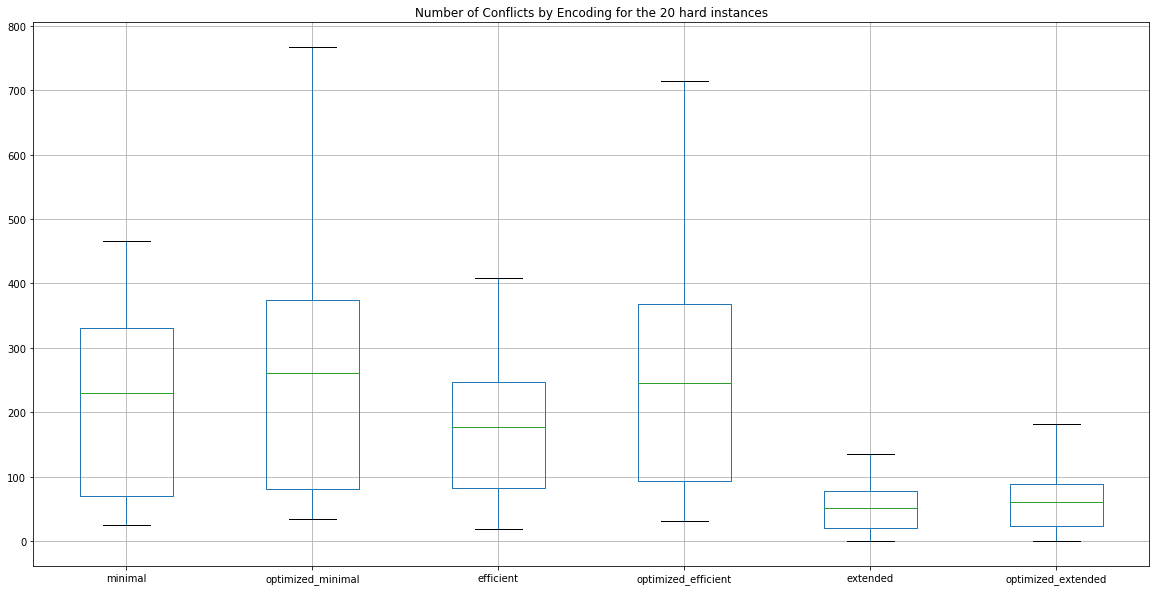
\includegraphics[scale=0.25]{report/conflicts}
\caption{Graph of the conflicts}
\end{figure}
\end{frame}


\subsection{Restarts}
\begin{frame}{Restarts}
\begin{figure}
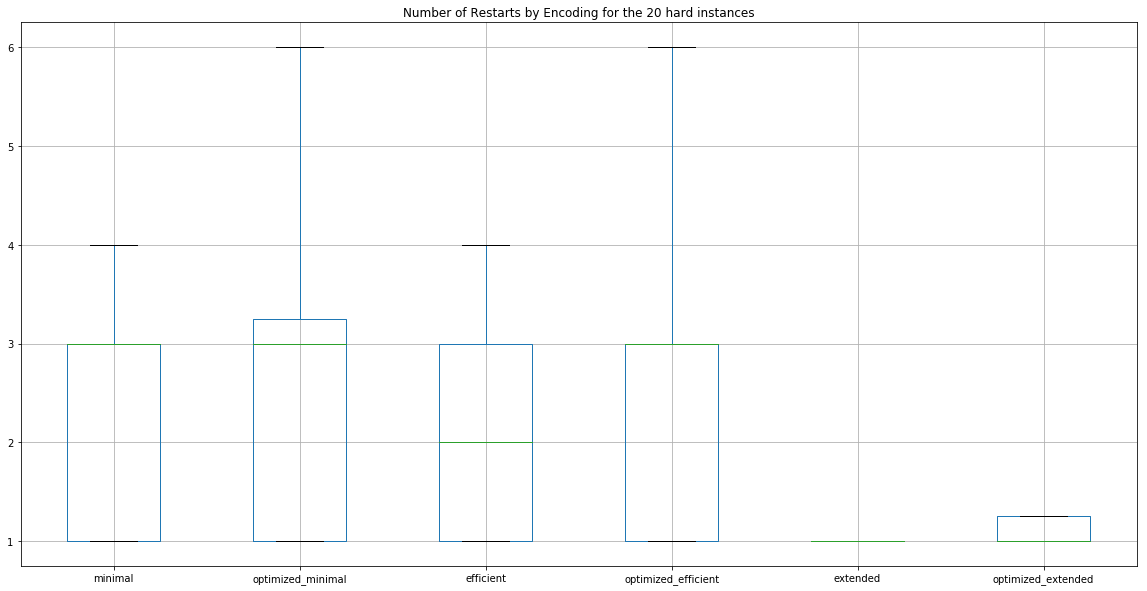
\includegraphics[scale=0.25]{report/restarts}
\caption{Graph of the restarts}
\end{figure}
\end{frame}

\subsection{Decisions}
\begin{frame}{Decisions}
\begin{figure}
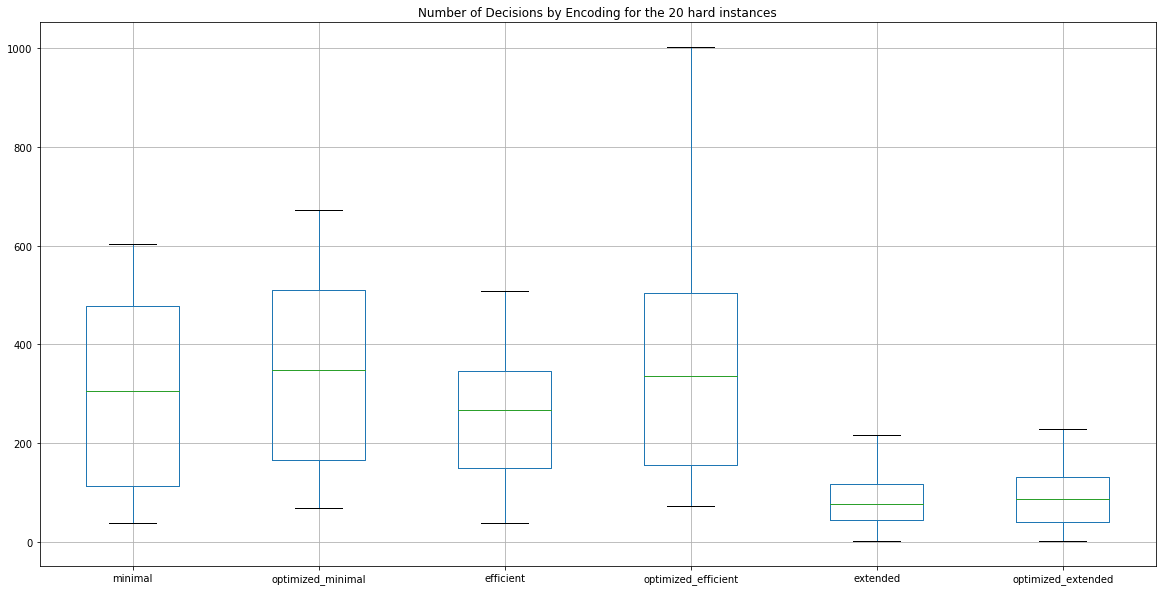
\includegraphics[scale=0.25]{report/decisions}
\caption{Graph of the decisions}
\end{figure}
\end{frame}

\subsection{Propagations}
\begin{frame}{Propagations}
\begin{figure}
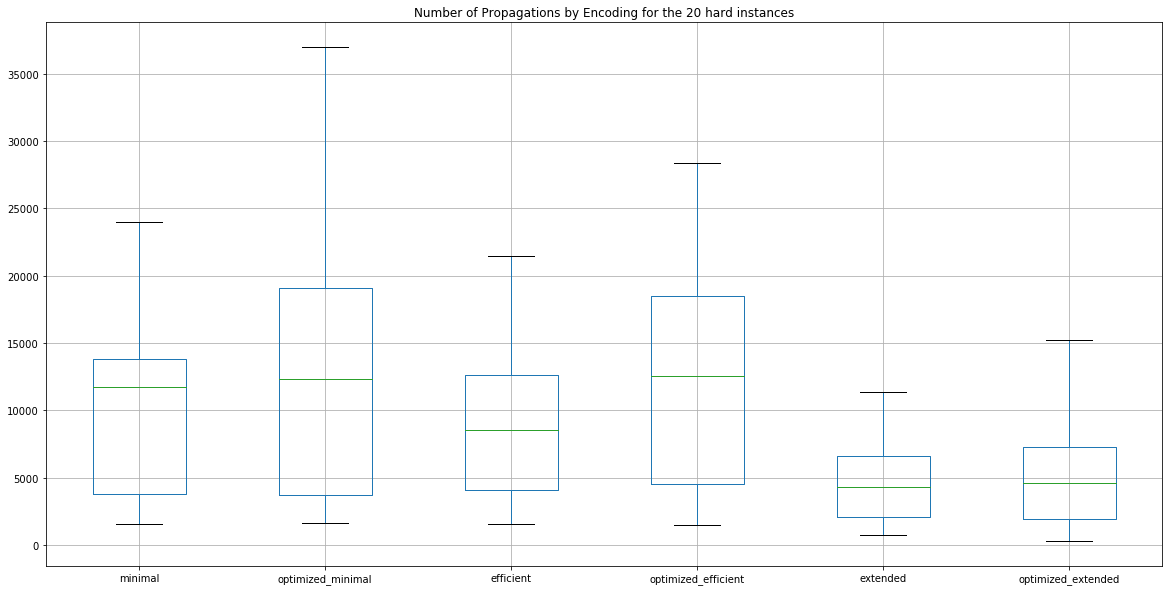
\includegraphics[scale=0.25]{report/propagations}
\caption{Graph of the propagations}
\end{figure}
\end{frame}

\subsection{Conflict Literals}
\begin{frame}{Conflict Literals}
\begin{figure}
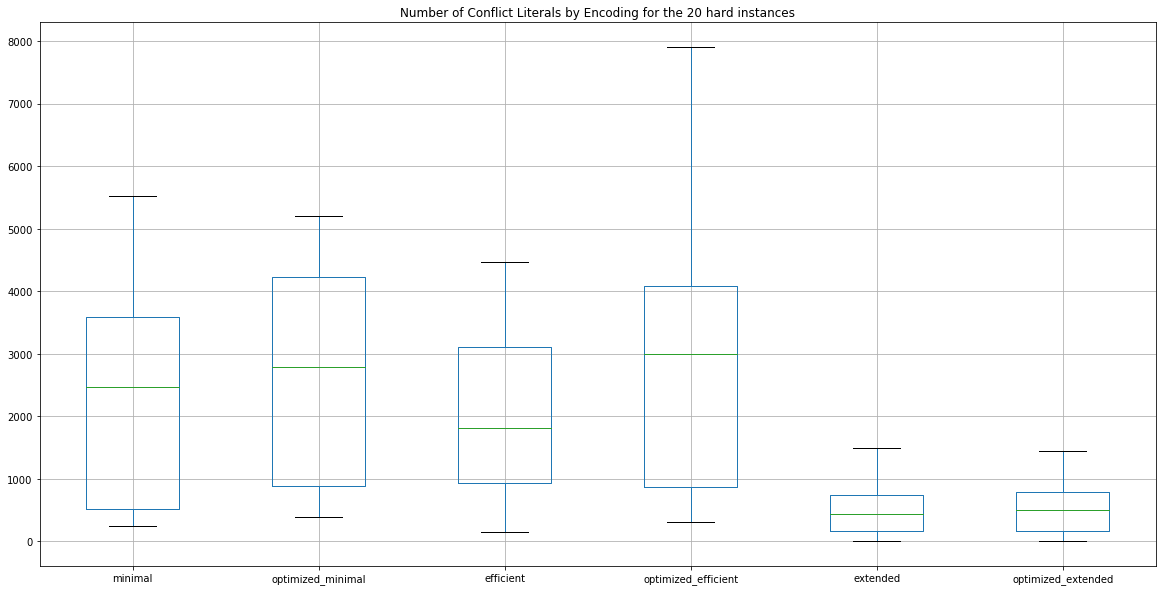
\includegraphics[scale=0.25]{report/conflict_literals}
\caption{Graph of the conflict literals}
\end{figure}
\end{frame}


\end{document}
